\documentclass[a4paper]{article}

\usepackage[polish]{babel}
\usepackage[utf8]{inputenc}
\usepackage[T1]{fontenc}
\usepackage{graphicx}
\graphicspath{ {./aem/} }
\usepackage[colorinlistoftodos]{todonotes}
\usepackage[procnames]{listings}
\usepackage{ucs}
\usepackage{float}
\usepackage{hyperref}


\lstset{
    basicstyle=\ttfamily\small,
    numberstyle=\footnotesize,
    numbers=left,
	frame=single,
    tabsize=2,
    rulecolor=\color{black!30},
    breaklines=true,
    breakatwhitespace=true,
    inputencoding=utf8x,
    extendedchars=\true,
    literate={ą}{{\k{a}}}1
             {Ą}{{\k{A}}}1
             {ę}{{\k{e}}}1
             {Ę}{{\k{E}}}1
             {ó}{{\'o}}1
             {Ó}{{\'O}}1
             {ś}{{\'s}}1
             {Ś}{{\'S}}1
             {ł}{{\l{}}}1
             {Ł}{{\L{}}}1
             {ż}{{\.z}}1
             {Ż}{{\.Z}}1
             {ź}{{\'z}}1
             {Ź}{{\'Z}}1
             {ć}{{\'c}}1
             {Ć}{{\'C}}1
             {ń}{{\'n}}1
             {Ń}{{\'N}}1
}

\title{Problem komiwojażera}

\author{Adrian Stępień i Wojciech Młyńczak}

\begin{document}

\maketitle

\section{Opis zadania}

\paragraph{}
Rozważany problem to zmodyfikowany problem komiwojażera. Dany jest zbiór wierzchołków i macierz odległości pomiędzy każdą parą wierzchołków. Celem zadania jest znalezienie najkrótszej ścieżki zamkniętej przechodzącą przez 50\% wszystkich wierzchołków (w przypadku nieparzystej liczby wierzchołków liczba jest zaokrąglana w górę).

\section{Opis zaimplementowanych algorytmów}

\subsection{Algorytm zachłanny greedy cycle}

\begin{lstlisting}
Wybierz pierwszy punkt.
Wybierz drugi punkt leżący najbliżej pierwszego.
Jeżeli nie dodałeś wszystkich punktów:
	Dla pozostałych wolnych punktów:
		Dla każdej krawędzi w aktualnym rozwiązaniu:
			Oblicz koszt dodania punktu do rozwiązania w danej krawędzi.
			Sprawdź czy to jest najlepsze rozwiązanie w danym momencie.
	Dodaj znaleziony najlepszy punkt w wybranej krawędzi do cyklu.
\end{lstlisting}

\subsection{Algorytm z żalem oparty o 1-żal}

\begin{lstlisting}
Wybierz pierwszy punkt.
Wybierz drugi punkt leżący najbliżej pierwszego.
Jeżeli nie dodałeś wszystkich punktów:
	Dla pozostałych wolnych punktów:
		Dla każdej krawędzi w aktualnym rozwiązaniu:
			Oblicz koszt dodania punktu do rozwiązania w danej krawędzi.
			Dodaj punkt do listy potencjalnych rozwiązań wraz z kosztem dodania.
		Oblicz żal dla danego punktu
	W liście potencjalnych rozwiązań znajdź rozwiązanie z największym żalem.
	Dodaj znalezione rozwiązanie z największym żalem do cyklu.
\end{lstlisting}

\section{Wyniki pomiarów}

\subsection{Algorytm zachłanny dla problemu kroA100}

\begin{center}
	\begin{tabular}{ l | l }
		\textbf{Pomiar} & \textbf{Wynik} \\
		\hline
		Wartość średnia    & 12898.45 \\
		Wartość minimalna  & 11325.00 \\
		Wartość maksymalna & 14067.00 \\
	\end{tabular}
\end{center}

\subsection{Algorytm oparty o żal dla problemu kroA100}

\begin{center}
	\begin{tabular}{ l | l }
		\textbf{Pomiar} & \textbf{Wynik} \\
		\hline
		Wartość średnia    & 16879.11 \\
		Wartość minimalna  & 14456.00 \\
		Wartość maksymalna & 17899.00 \\
	\end{tabular}
\end{center}

\subsection{Algorytm zachłanny dla problemu kroB100}

\begin{center}
	\begin{tabular}{ l | l }
		\textbf{Pomiar} & \textbf{Wynik} \\
		\hline
		Wartość średnia    & 12710.59 \\
		Wartość minimalna  & 10240.00 \\
		Wartość maksymalna & 11320.00 \\
	\end{tabular}
\end{center}

\subsection{Algorytm oparty o żal dla problemu kroB100}

\begin{center}
	\begin{tabular}{ l | l }
		\textbf{Pomiar} & \textbf{Wynik} \\
		\hline
		Wartość średnia    & 17245.51 \\
		Wartość minimalna  & 15547.00 \\
		Wartość maksymalna & 16965.00 \\
	\end{tabular}
\end{center}

\section{Wizualizacje najlepszych rozwiązań}

\subsection{Algorytm zachłanny dla problemu kroA100}

\begin{figure}[H]
\centering
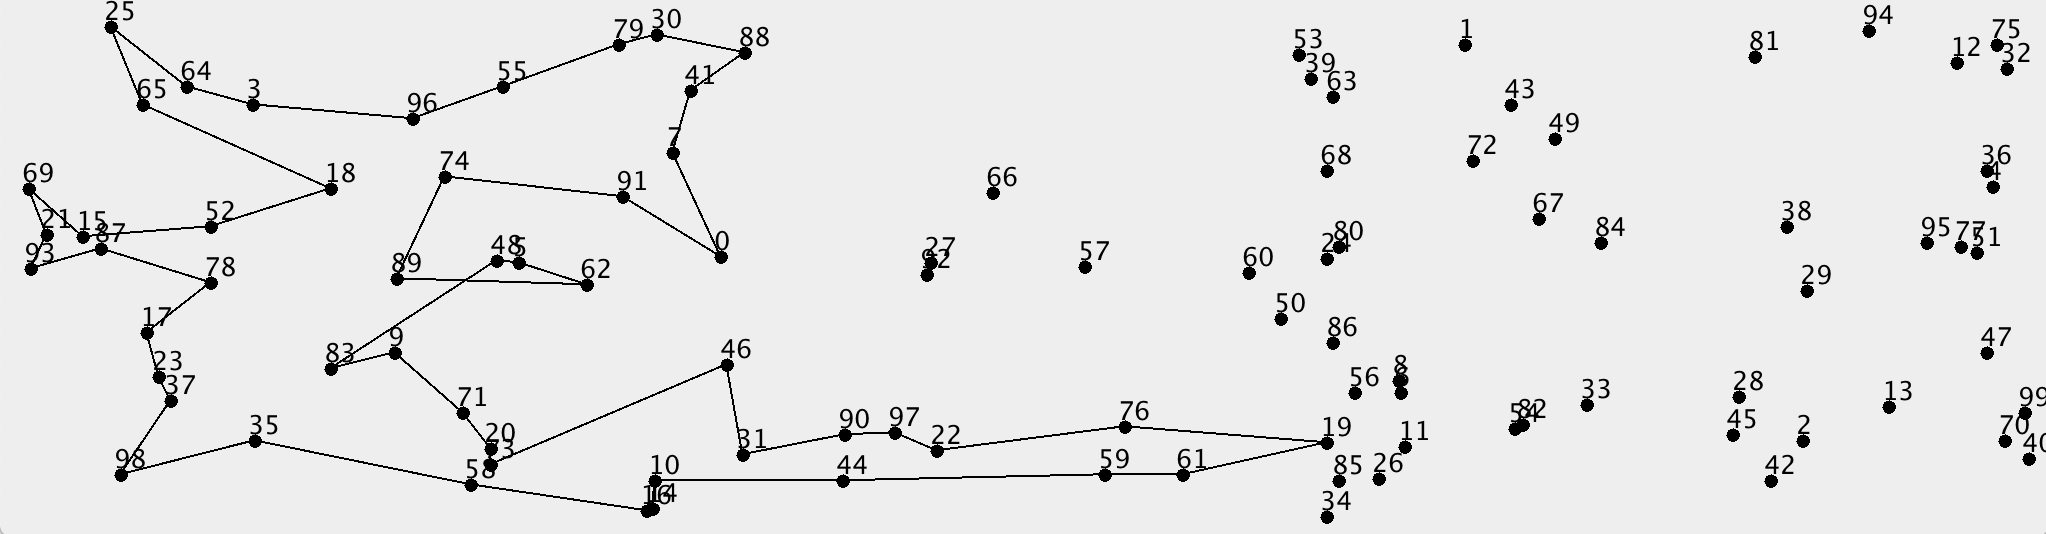
\includegraphics[width=\textwidth]{kroA_greedy}
\caption{Algorytm zachłanny dla problemu kroA100}
\end{figure}

\subsection{Algorytm oparty o żal dla problemu kroA100}

\begin{figure}[H]
\centering
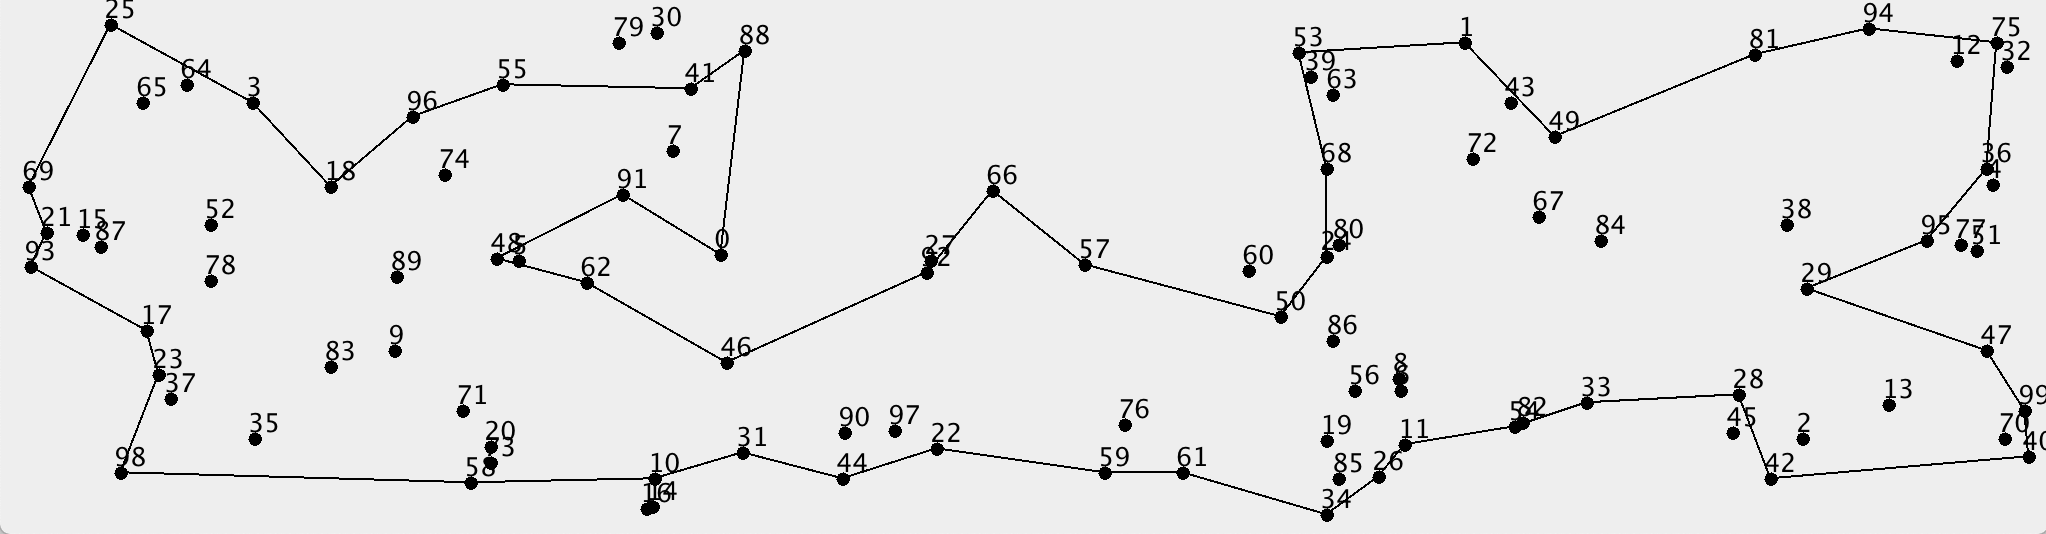
\includegraphics[width=\textwidth]{kroA_regret}
\caption{Algorytm oparty o żal dla problemu kroA100}
\end{figure}

\subsection{Algorytm zachłanny dla problemu kroB100}

\begin{figure}[H]
\centering
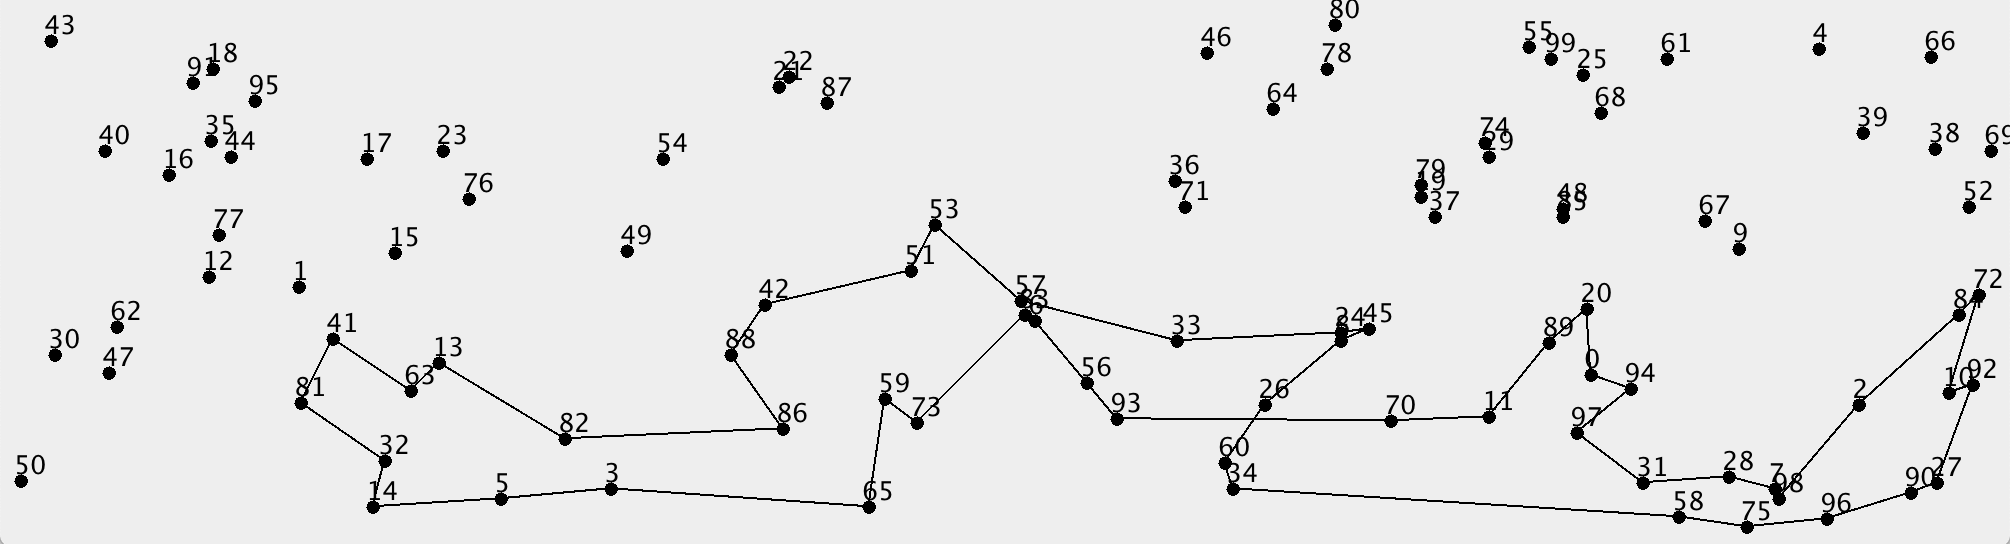
\includegraphics[width=\textwidth]{kroB_greedy}
\caption{Algorytm zachłanny dla problemu kroB100}
\end{figure}

\subsection{Algorytm oparty o żal dla problemu kroB100}

\begin{figure}[H]
\centering
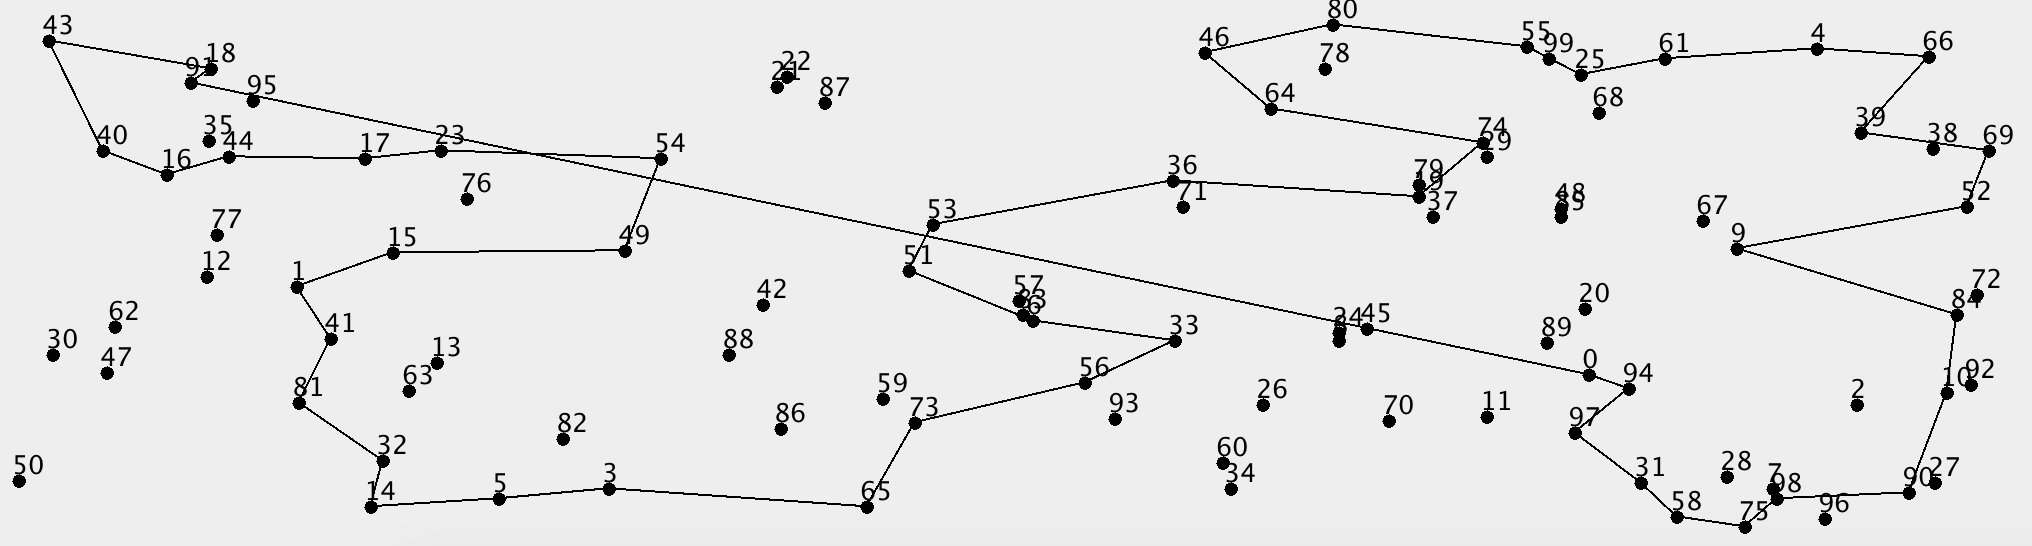
\includegraphics[width=\textwidth]{kroB_regret}
\caption{Algorytm oparty o żal dla problemu kroB100}
\end{figure}

\section{Wnioski}
\paragraph{}
Z wymienionych wyżej pomiarów można wywnioskoważ, że dla podanych warunków problemu (odwiedzanie połowy punktów), algorytm zachłanny radzi sobie lepiej od algorytmu opartego o żal (cykl, który generuje ma mniejszą długość). Przeprowadzono również testy dla przypadku, gdy oba te algorytmy uruchomione zostaną dla wszystkich punktów. Wtedy wyniki są odmienne, algorytm z żalem okazuje się lepszy od algorytmu zachłannego. Jest to spowodowane tym, że dla warunków zadania z odwiedzeniem połowy punktów algorytm z żalem czasami dodaje punkty, które mają duży żal, a w ogóle nie powinny zostać dodane do cyklu z powodu dużego kosztu ich dodania. Gdy odwiedzone mają być wszystkie punkty, koszt dodania punktu nie ma takiego znaczenia, ponieważ prędzej lub później i tak każdy punkt będzie musiał zostać dodany. 

\section{Kod programu}
\paragraph{}
Repozytorium z kodem programu dostępne jest pod adresem: \url{https://github.com/adrianstepienfsw/AEM1}

\end{document}